\documentclass[convert]{standalone}
\usepackage{tikz} 
\usetikzlibrary{graphs} 
\usetikzlibrary{positioning} 
\usetikzlibrary{arrows.meta}
\begin{document}

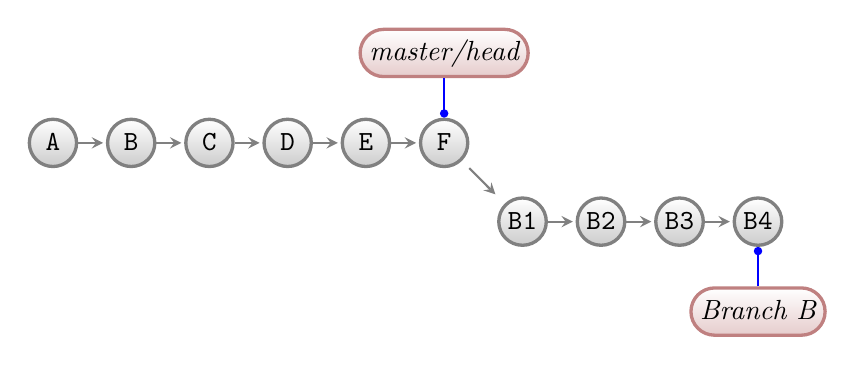
\begin{tikzpicture}[
nonterminal/.style={
	% The shape:
	rectangle,
	% The size:
	minimum size=6mm,
	% The border:
	very thick,
	draw=red!50!black!50, % 50% red and 50% black,
	% and that mixed with 50% white
	% The filling:
	top color=white, % a shading that is white at the top...
	bottom color=red!50!black!20, % and something else at the bottom
	% Font
	font=\itshape},
every node/.style={
	% The shape:
	rectangle,minimum size=6mm,rounded corners=3mm,
	% The rest
	very thick,draw=black!50,
	top color=white,bottom color=black!20,
	font=\ttfamily},
text height=1.5ex,text depth=.25ex,
>=stealth, thick, black!50, text=black,
every new ->/.style={shorten >=1pt},
graphs/every graph/.style={edges=rounded corners},
]

\graph [grow right sep] { A -> B -> C -> D -> E -> F -> {
	   / [draw=none,top color=white,bottom color=white,not source],
	   B1 -> B2 -> B3 -> B4
	 } 
};

%\node (head) [node distance=5mm, nonterminal,above =of B4] {head};
%\draw[-{Circle[length=3pt]},blue] (head) -- (B4);
\node (master) [node distance=5mm, nonterminal,above =of F] {master/head};
\draw[-{Circle[length=3pt]},blue] (master) -- (F);
\node (Branch B) [node distance=5mm, nonterminal,below =of B4] {Branch B};
\draw[-{Circle[length=3pt]},blue] (Branch B) -- (B4);

\end{tikzpicture}

\end{document}
